%%%%%%%%%%%%%%%%%%%%%%%%%%%%%%%%%%%%%%%%
%%% aims of the NEXT-Tonne UTA workshop
%%% J. Martin-Albo, A. Laing 2019
%%% NEXT Collaboration

\documentclass[11pt,a4paper]{article}
\usepackage[a4paper,vmargin={1.0cm,1.5cm},width=18cm]{geometry}

\usepackage{multirow}
\usepackage{amsmath,amssymb, gensymb}
\usepackage{graphicx}
\usepackage{textcomp}

\begin{document}

\title{Aims of the NEXT-Tonne UT Arlington workshop}

\maketitle

\abstract{The NEXT collaboration has demonstrated the strength of gaseous xenon TPCs with electroluminescent amplification as a technology for the observation of neutrino-less double beta decay. The first results using xenon enriched to 91\% in the double beta isotope are due in 2019 with the 100~kg scale detector due to come online in 2020. This workshop aims to select baseline designs for a detector with fiducial mass in the region of 500 -- 1000~kg of xenon. Using simulated MC data we will assess the feasibility of baseline designs both in terms of size and of the technologies for the read-out of the detector.}

\section{Introduction}
A large mass NEXT-style detector would not only need to reach the required larger mass but significantly reduce expected backgrounds to be sensitive to effective masses over the whole parameter space allowed by the inverted hierarchy. In this workshop we will study the impact and feasibility of various changes to the materials and read-out technologies used with the aim of choosing baseline design(s) for more detailed study.

\section{Learning from NEW and NEXT-100}
In the current detectors the vessels are shielded from the lab using lead bricks which form a `castle' inside which air with reduced radon content is flowed. As we move to a greater mass of xenon, backgrounds induced by neutron interactions will become more important, as detailed in \cite{munozth:2018}. Placing the detector in a water tank will shield more effectively against neutrons but size and whether and how to instrument such a tank need to be studied in detail.


\section{Possible designs}
\label{sec:posdes}

\subsection{Design Ia: NEXT-500}
\label{subSec:desia}
The most basic imaginable large scale NEXT detector is a direct scale up of the current NEXT-100 design using the same technologies. This design has a number of possible problems:
\begin{itemize}
\item What coverage of PMTs is possible?
\item What density of tracking plane is feasible?
\item How can the radioactive budget be reduced?
\end{itemize}

\subsection{Design Ib: NEXT-SiPM}
\label{subSec:desib}
One way to significantly reduce expected radioactive budget is by replacing the PMTs with large surface area SiPMs without any other major geometrical changes. That is, still having separate planes for energy and topological reconstruction. The technological difficulties of this design would be:
\begin{itemize}
\item What level of DC is required for a reliable energy measurement?
\item Is this technologically achievable?
\item Can the SiPM response remain linear over the light levels necessary?
\item Can S1 be efficiently detected?
\end{itemize}

\subsection{Design II: NEXT-SinglePlane}
\label{subSec:desii}
Another possible design would mix SiPMs of various surface areas in the plane behind the EL region where both energy and topology reconstructions will be performed. In this way the cathode side is free for use for other possible functions. This design suffers from the same problems as design {\bf Ib} with the solution of the linearity problem being even more crucial since light at the EL plane is more focused and intense.

\subsection{Design III: NEXT-symmetric}
\label{subSec:desiii}
A symmetric design with the same readout as design {\bf II} is also possible which would reduce the maximum drift for the same detector length. This design would have similar difficulties to the previous two.

\subsection{Additional improvements}
\label{subSec:desadd}
In basically all the designs mentioned above there are some additional technological additions that could improve light collection.

The SiPM-wheel design would instrument the edges of the solid anode plate and collect internally reflected light. This could improve reconstruction at high radii as well as improving photon statistics/effective coverage of sensors for the energy reconstruction.

The light tube could also be directly instrumented, most likely using wavelength shifting fibres or other light concentrators which would collect light and guide it either to behind the copper support plates or outside the detector. In this way, the effect of radioisotopes in the materials of any sensor used to read out the signal would have a significantly reduced impact on the active volume. This design could have a significant effect on light collection for the detection of primary scintillation.

\section{Detector size}
\label{sec:size}

\subsection{Fiducial mass}
\label{subSec:fidmass}
A fiducial mass of approximately 500~kg per module will be required to achieve a competitive but stageable design. In real terms this translates to the dimensions shown in table~\ref{tab:mass} for the desings mentioned in section \ref{sec:posdes}.
\begin{table}
  \begin{center}
    \begin{tabular}{|l|c|c|c|c|c|c|}
      \hline
      \multirow{2}{*}{} & \multirow{2}{*}{Length (m)} & \multirow{2}{*}{Diameter (m)} & \multirow{2}{*}{Volume (m$^3$)} & \multicolumn{2}{c|}{Xe mass (kg)} & \multirow{2}{*}{Symmetric?} \\
      \cline{5-6}
                        & & & & 10 bar, 300 K & 15 barm 300 K & \\
      \hline
      NEXT-White & 0.530 & 0.454 & 0.086 &     5 &     7 &  NO \\
      NEXT-100    & 1.160 & 1.010 & 0.929 &   52 &   80 &  NO \\
      NEXT-T Ia    & 3.000 & 1.500 & 5.301 & 295 & 456 &  NO \\
      NEXT-T Ib    & 3.000 & 1.500 & 5.301 & 295 & 456 &  NO \\
      NEXT-T II     & 3.000 & 1.500 & 5.301 & 295 & 456 &  NO \\
      NEXT-T III    & 5.000 & 1.500 & 8.836 & 491 & 759 & YES \\
    \hline
    \end{tabular}
  \end{center}
  \caption{\label{tab:mass} Dimensions and approximate active masses for the basic designs}
\end{table}
Using these basic designs as a guide it is clear that 15~bar operation is favoured from the point of view of achieving a competitive mass in a reasonably sized pressure vessel. 

\subsection{Drift length}
\label{subSec:drift}
The maximum drift length for the detector designs is 3~m for the asymmetric TPCs and 2.5~m for the symmetric design. Assuming that electron lifetime can, at least, reach the levels recorded currently in NEXT-White, $\tau \simeq 5$~ms, and that the drift velocity in the TPC will be of order 1~mm~\textmu s$^{-1}$, at worst we would expect the S2 signals at maximum drift to have ~55\% of the charge of minimum drift events for the asymmetric design and ~61\% in the case of a symmetric TPC.

The main limiting factors of the electron lifetime in NEXT-White have been identified as turbulent flow of the gas in the active volume coupled with virtual leaks and outgasing from the plastics after exposure to laboratory air. In NEXT-100 the gas flow has been studied more extensively so as to limit the effect of turbulence. Moreover, clean room facilities will be installed on the NEXT platform, limiting the movements required and possible exposure of the inner detector materials to laboratory air. The issue will be studied extensively in NEXT-100 but there doesn't seem to be any good reason why the level of purity  won't be as good or better in a larger detector and, as such, should not be a problem.

\section{Limiting factors}
\label{sec:limit}
There are number of possible limiting factors for a feasible design. Initial studies will focus on understanding these limitations in order to reject any design unable to deal with them.

\subsection{S1 detection}
\label{subSec:S1det}
Detection of primary scintillation constitutes the smalles signals that must be detected efficiently in any NEXT detector. In the asymmetric, split functions designs ({\bf Ia, Ib}) events close to the anode will be the most difficult to detect while for designs {\bf II \& III} it would be those close to the cathode.

If we assume an interaction at the maximum distance from the detection plane and that no reflection is possible we only need consider the solid angle subtended by the detection plane, the proportional coverage of sensitive detectors, the conversion efficiency to the blue, and the photon detection efficiency of the sensors in order to determine the proportion of the scintillation photons we would expect to detect. While this is, of course, overly conservative an optical simulation would be required (and will be performed) to fully appreciate this requirement. For now we will limit ourselves to this basic calculation and an empirical scaling based on observations in NEXT-White and NEXT-DEMO. In summary, we expect the number of photons to be detected (before taking into account reflections) to be described by:
\begin{equation}
  \label{eq:s1npe}
  n_{pe} = n_{phot} \cdot \frac{\omega}{4\pi} \cdot c \cdot eff_{TPB} \cdot PDE,
\end{equation}
where $n_{pe}$ is the number of photoelectrons detected, $\omega$ is the solid angle subtended by the detection plane, $c$ is the proportional coverage with sensitive detectors, $eff_{TPB}$ is the conversion efficiency of the TPB and $PDE$ is the photon detection efficiency of the sensors (or sensor systems). For an event in the middle of the furthest plane from the detection plane the solid angle subtended is:
\begin{equation}
  \label{eq:s1solidangle}
  \omega = 4\pi \mbox{sin}^2\frac{\theta}{2} = 4\pi \mbox{sin}^20.5\cdot(\mbox{tan}^{-1}\frac{r}{d}),
\end{equation}
where $r$ is the radius of the detector active volume and $d$ is the drift length. Table \ref{tab:s1phot} summarieses the $n_{pe}$ as calculated for the existing detectors and the baseline tonne scale designs for a Kr event in the centre of the plane furthest from the detection plane. We assume that a Kr event produces approximately 650 scintillation photons in all cases. For the coverage with PMTs we assume 30\% as in NEXT-White and for SiPM designs we assume sensors with active surfaces of $3\times 3~\mbox{mm}^2$ spaced with a pitch of 1~cm in X and Y.
\begin{table}
  \begin{center}
    \begin{tabular}{|l|c|c|c|c|}
      \hline
      Detector & \% sensor coverage & $\omega$ & $n_{phot}$ Kr & $n_{phot}^{\prime}$ Kr \\
      \hline
      NEXT-NEW & 30 & 0.51 &            1.18 &    3--4  \\
      NEXT-100  & 30 & 0.52 &            1.22 &    3--4   \\
      NEXT-T Ia  & 30 & 0.19 &            0.44 & 1.3--1.8 \\
      NEXT-T Ib  &   9 & 0.19 &            0.22 & 0.7--0.9 \\
      NEXT-T II   &   9 & 0.19 &            0.22 & 0.7--0.9 \\
      NEXT-T III  &   9 & 0.26 & 0.31--0.62 & 0.9--2.5 \\
      \hline
    \end{tabular}
  \end{center}
  \caption{\label{tab:s1phot} Estimations of the number of available photons at the detection plane for various NEXT detectors.}
\end{table}
In order to calculate $n_{phot}^{\prime}$ we use a scaling factor of 3--4 times based on the minimum Kr S1 signal seen in NEXT-White compared to the $n_{phot}$ value calculated here (see figure \ref{fig:news1}).
\begin{figure}
  \begin{center}
    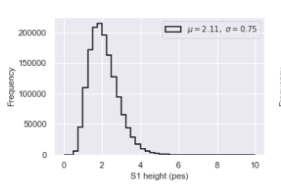
\includegraphics[width=0.49\textwidth]{img/NEW_s1_eng}
  \end{center}
  \caption{\label{fig:news1} Distribution of summed pmt signal for Kr S1 in NEW.}
\end{figure}
Such low levels of light dictate the quality of the sensors. While PMTs should be able to unambiguously detect a few photons the challenge is greater with SiPMs due to non-negligible levels of thermal excitation. These dark counts could mimick an S1 in a plane with many sensors. In order to be able to use SiPMs for this measurement we must understand the limitations of the technology by calculating the probability of mimicking an S1 for available technology as well as what reduction in dark counts would be required to make the experiment possible.

Current large surface area models of SiPMs have DC rates of approximately 0.5~counts~\textmu s$^{-1}$. If, like in NEXt-White, we sample at 1~MHz (every \textmu s) that means that there would be a probability 50\% to produce a fake pe every sample.
%The lowest light level that will need to be detected is the S1 produced by Kr used for the point calibration of the detector response.

\bibliographystyle{unsrt}
\bibliography{refs}

\end{document}